% $File: report.tex
% $Date: Sat Sep 15 23:33:21 2012 +0800
% $Author: wyx <ppwwyyxxc@gmail.com>

\documentclass[a4paper]{article}
\usepackage{fontspec,amsmath,amssymb,zhspacing,minted}
\usepackage[hyperfootnotes=false,colorlinks,linkcolor=blue,anchorcolor=blue,citecolor=blue]{hyperref}
\usepackage[sorting=none]{biblatex}
%\usepackage[dvips]{graphicx}
\usepackage{indentfirst}
\newfontfamily\zhfont[BoldFont=SimHei,ItalicFont=KaiTi_GB2312]{SimSun}
\zhspacing

\renewcommand{\abstractname}{摘要}
\renewcommand{\contentsname}{目录}
\renewcommand{\figurename}{图}
\defbibheading{bibliography}{\section{参考文献}}
\bibliography{refs.bib}

% \figref{label}: reference to a figure
\newcommand{\figref}[1]{\hyperref[fig:#1]{图\ref*{fig:#1}}}
% \secref{label}: reference to a section
\newcommand{\secref}[1]{\hyperref[sec:#1]{\ref*{sec:#1}节}}
\DeclareMathOperator{\rank}{\tiny{rank}}

\let\Oldsum\sum
\renewcommand{\sum}{\displaystyle\Oldsum}
\let\Oldprod\prod
\renewcommand{\prod}{\displaystyle\Oldprod}

% $File: mint-defs.tex
% $Date: Sat Feb 16 22:59:11 2013 +0800
% $Author: wyx <ppwwyyxxc@gmail.com>

\usepackage{xparse}


% \inputmintedConfigured[additional minted options]{lang}{file path}{
\newcommand{\inputmintedConfigured}[3][]{\inputminted[fontsize=\footnotesize,
	label=#3,linenos,frame=lines,framesep=0.8em,tabsize=4,#1]{#2}{#3}}

% \phpsrc[additional minted options]{file path}: show highlighted php source
\newcommand{\phpsrc}[2][]{\inputmintedConfigured[#1]{php}{#2}}
% \phpsrcpart[additional minted options]{file path}{first line}{last line}: show part of highlighted php source
\newcommand{\phpsrcpart}[4][]{\phpsrc[firstline=#3,firstnumber=#3,lastline=#4,#1]{#2}}
% \phpsrceg{example id}
\newcommand{\phpeg}[1]{\inputminted[startinline,
	firstline=2,lastline=2]{php}{res/php-src-eg/#1.php}}

\newcommand{\txtsrc}[2][]{\inputmintedConfigured[#1]{text}{#2}}
\newcommand{\txtsrcpart}[4][]{\txtsrc[firstline=#3,firstnumber=#3,lastline=#4,#1]{#2}}

\newcommand{\pysrc}[2][]{\inputmintedConfigured[#1]{py}{#2}}
\newcommand{\pysrcpart}[4][]{\pysrc[firstline=#3,firstnumber=#3,lastline=#4,#1]{#2}}

\newcommand{\confsrc}[2][]{\inputmintedConfigured[#1]{squidconf}{#2}}
\newcommand{\confsrcpart}[4][]{\confsrc[firstline=#3,firstnumber=#3,lastline=#4,#1]{#2}}

\newcommand{\cppsrc}[2][]{\inputmintedConfigured[#1]{cpp}{#2}}
\newcommand{\cppsrcpart}[4][]{\cppsrc[firstline=#3,firstnumber=#3,lastline=#4,#1]{#2}}

\renewcommand{\P}[1]{\text{P}\left(#1\right)}
\renewcommand{\Pr}[1]{\text{Pr}\left\{#1\right\}}
\newcommand{\Px}[2]{\text{P}_{#1}\left(#2\right)}
\newcommand{\E}[1]{\text{E}\left[#1\right]}
\newcommand{\Ex}[1]{\text{E}#1}
\newcommand{\Var}[1]{\text{Var}\left[#1\right]}
%\newcommand{\Cov}[2]{\text{Cov}\left[#1,#2\right]}
%\newcommand{\Cov}[1]{\text{Cov}\left[#1 \right]}
\renewcommand{\T}[1]{\Theta\left(#1\right)}
\newcommand{\real}{\mathbb{R}}
\newcommand{\card}[1]{\left\|#1\right\|}
\newtheorem{lemma}{Lemma}

\NewDocumentCommand\Cov{mg}{
    \text{Cov}\left[ #1 \IfNoValueTF{#2}{}{,#2}\right]
 }

\newcommand{\qed}{\hfill \ensuremath{\Box}}



\title{线性代数与多项式方程组求解}
\date{}

\begin{document}
\maketitle

\tableofcontents
\nocite{adv_alg}\nocite{ideals}\nocite{using}\nocite{lc}\nocite{poly_alg}
% File: intro.tex
% Date: Wed Jul 17 14:44:12 2013 +0800
% Author: Yuxin Wu <ppwwyyxxc@gmail.com>

\section{Introduction}
Let $ \pi= (\pi(1), \pi(2),\cdots ,\pi(n))$ be a permutation of $ (1,2,\cdots ,n)$.
The \emph{Fixed Points} of the permutation $ \pi$ ,
denoted as $ \mathcal{F}(\pi)$, is defined as follows:
\[ \mathcal{F}(\pi) = \{ k \in [1,n]\cap \mathbb{N} \mid \pi(k) = k \}\]

Let $ \Pi_n$ be the set of all possible permutations of $ (1,2,\cdots ,n)$.
The \emph{Rencontres Numbers}\cite{wiki_rn}
$ D_{n,k}$ is defined as follows:
\[ D_{n,k} = \card{ \{ \pi \in \Pi_n \mid \card{\mathcal{F}(\pi)} = k \}}, k = 0,1,\cdots n\]
where $ \card{A}$ is the cardinality of a set $ A$.

In particular, we denote $ D_{n,0}$ as $  D_{n} $ for short.

Let $ \pi $ be a random permutation of $ (1,2,\cdots ,n),$ where
every possible permutation has the same possibility $ \dfrac{1}{n!}$.
The random variable $ X = \card {\mathcal{F}(\pi)} $ is what we will focus on in this paper.


% $File: resultant.tex
% $Date: Sat Jun 02 17:24:14 2012 +0800
% Author: WuYuxin <ppwwyyxxc@gmail.com>
\section{结式方法}
\subsection{原理}
	消元是解方程组的基本原理.
	对于解线性方程组,由于方程只有一次,可以直接将每个方程中的一变元用其余变元表出,再代入消元.
	但对于多项式方程组,由于很多类型的高次方程无根式解,即使有也大多极其复杂,难以使用传统的代入消元手段进行消元,
	而基于换元或方程相加减等的消元方法太过于依赖结构,不具有计算机处理所需的通用性.
	因此需要引入其他的消元方法,结式(Resultant)就是一种.

	首先考虑复数域上关于$ x$的两个多项式方程构成的方程组
	\[  \begin{cases} 
			f(x)=\sum_{i=0}^{n}{a_ix^{n-i}}=0 \\
			g(x)=\sum_{i=0}^{m}{b_ix^{m-i}}=0
	\end{cases} , \texttt{其中} a_0b_0\ne0\]

	这个方程组的解,实际上就是指两多项式的公共复根.

	$ f(x)=0,g(x)=0$有公共复根

	$ \Leftrightarrow \exists f_1(x), g_1(x), \deg f_1(x) < n, \deg g_1(x) < m, \dfrac{f(x)}{f_1(x)} = \dfrac{g(x)}{g_1(x)}$

	$ \Leftrightarrow \exists f_1(x),g_1(x),\deg f_1(x)<n,\deg g_1(x)<m,f(x)g_1(x)=g(x)f_1(x)$

	于是设$ f_1(x)=\sum_{i=0}^{n-1}{u_ix^{n-1-i}},g_1(x)=\sum_{i=0}^{m-1}{v_ix^{m-1-i}}$,
	代入上式,比较左右两边所有$ m+n$个项的系数,可得$ m+n$个线性方程.

	\[ \left \{  \begin{array}{lrclr}
	a_0v_0		&			&= &b_0u_0		&		\\
	a_1v_0+a_0v_1&			&= &b_1u_0+b_0u_1&		\\
	\cdots \cdots &\cdots	&= & \cdots\cdots &\cdots		\\
			&{a_nv_{m-2}+a_{n-1}v_{m-1}}&=&		&b_mu_{n-2}+b_{m-1}u_{n-1}\\
			& a_nv_{m-1}&= &				&b_mu_{n-1}\\
	\end{array}\right . \]

	这个关于$(v_0,\cdots,v_{m-1},u_0,\cdots,u_{n-1})$ 的$ m+n$元齐次线性方程组必须有非零解
	,于是其系数行列式
	
	\[ A=\begin{vmatrix} 
		a_0	&	&	&	&	 &		& b_0 &		&	 &	\\
		a_1	&a_0&	&	&			&	& b_1 & b_0	&	&	\\
  \cdots &\cdots &\cdots &\cdots	&  \cdots&	& \cdots &\cdots	&	\cdots	&	\\
		 &	&	&	&a_n &a_{n-1}   &		&	& b_m  & b_{m-1} \\
		 &	&	&	&	 &a_n		&		&	&	  & b_m\\
	\end{vmatrix} = 0\]

	也即其转置
	\[A^{T}= \begin{vmatrix}
	a_0 & a_1 & \cdots & \cdots & \cdots & \cdots & a_n		&		&	&   \\
		& a_0 & a_1	   & \cdots & \cdots & \cdots & \cdots  &a_n   &	&	\\
		&	  & \cdots & \cdots & \cdots & \cdots & \cdots &		&	&	\\
		&	  &		   & a_0	& a_1	 & \cdots & \cdots & \cdots &	& a_n\\
	b_0 & b_1 & \cdots & b_m	&		 &		  &		   &		&	&   \\
		& b_0 & b_1	   & \cdots  &b_m   &	    	&		&		&	&	\\
		&	  & \cdots & \cdots & \cdots & \cdots & \cdots &		&	&	\\
		&	  &		   &		&		&		& b_0		& b_1	& \cdots & b_m\\
	\end{vmatrix} =0\]
	注意到$ A^{T}$仅由多项式$ f,g$的系数决定,可记$ Res_x(f,g)=|A^{T}|,$
	称其为多项式$ f,g$的{\bf Sylvester结式(Sylvester's Resultant) },简称结式.

	根据上述讨论,我们有结论:$ f(x),g(x)$有重根$ \Leftrightarrow Res_x(f,g) = 0$
	
	\vspace{13pt}
	再考虑二元多项式方程组:

	$ \begin{cases}
		f(x,y)=0 \\g(x,y)=0 
	\end{cases}$,以$ x$为主元,视$ y$为常数,可求得结式$ P(y) = R_x(f,g)$,是$ y$的多项式.

	由之前对一元方程组的讨论可知,对$ P(y)$的每个零点$ y_0,f(x,y_0),g(x,y_0)$有公共复根.
	反之,对于原方程组的每个解$ (x_0,y_0), $必有$ P(y_0) = 0$

	于是,对原方程组的求解转化为对一元方程$ P(y) = 0$的求解,成功实现了消元,降低了问题的难度.
	
	\vspace{13pt}
	对两个方程构成的含有多个变元的方程组,可以使用相同手段消去其中某个变元.
	而对于超过两个方程构成的方程组,可以每次取其中两个方程计算结式,例如解如下方程组:
	\[  \begin{cases} f_1 = xy+z-5 = 0\\ f_2 = x+y+z-6 = 0 \\ f_3 = x^2-2xy+y^2-2z = 0
	\end{cases}\]

	$ Res_x(f_1,f_2) = y^2+(z-6)y-z+5 $ 

	$ Res_x(f_2,f_3)=4y^2+(4z-24)y + z^2-14z+36$

	$ Res_y(Res_x(f_1,f_2),Res_x(f_2,f_3)) = (z-2)^2(z-8)^2$

	于是消去了$ y,z$,得到$ z=2,z=8,$代回原方程可求得完整解.

	对于多个方程构成的方程组,也有多元结式理论可以用于解决消元问题.\cite{ideals}

\subsection{应用}
	对于一元方程组,结式方法的一个重要应用是判断多项式是否有重根.
	考虑多项式$ f(x) = \prod_{i=1}^{k}{(x-x_i)^{r_i}}$,
	显然对于每个$ i$,有 $ r_i >1 \Leftrightarrow  f'(x_i) = 0 \Leftrightarrow x_i $ 是$f(x)$与$ f'(x)$的公共复根.
	所以, $ f(x)=0$有重根$ \Leftrightarrow Res(f,f')=0$.
	
	\vspace{5pt}
	另外,上述的二元方程组的结式求解方法可应用于物理解题中常常能遇到的一类代数曲面/曲线隐式化问题.
	例如,用参数方程表示的曲线
	$ \begin{cases}x=\dfrac{-t^2+2t}{t^2+1} \\ y=\dfrac{2t^2+2t}{t^2+1} \end{cases}$

	将两式都写为关于$ t$的多项式: 
	$\begin{cases}f(t)=(x+1)t^2 -2t +x\\ g(t)=(y-2)t^2-2t+y \end{cases}$

	排除掉$ x+1=y-2=0$的情形,计算结式$ Res_t(f,g)= 8x^2-4xy+5y^2+12x-12y$ 
	
	于是$8x^2-4xy+5y^2+12x-12y=0,(x,y) \ne (-1,2)$为曲线隐式化后的结果.

% $File: abstract.tex
% $Date: Tue May 29 11:12:55 2012 +0800
% Author: Yuxin Wu <ppwwyyxxc@gmail.com>
\section{抽象代数方法简述}
	本节主要将抽象代数方法里的一个基本概念与线性代数进行类比.
	为了求解线性方程组,我们首先学习了秩,线性相关等概念.

	对于方程组$ \begin{cases}
		f_1(x_1,\cdots,x_n)=0\\
		f_2(x_1,\cdots,x_n)=0\\
		f_3(x_1,\cdots,x_n)=0\\
		\vdots\\
	\end{cases}$
	
	它是一个线性方程组时,若$ f_3=p_1f_1+p_2f_2,p_1,p_2\in \mathbb{R}$,那么在原方程组中,$ f_3=0$是一个"没用"的方程.
	反映在对应的系数矩阵中,
	设$ \overrightarrow b_1,\overrightarrow b_2,\cdots $为行向量,则
	$ \overrightarrow b_3$可由$ \overrightarrow b_1,\overrightarrow b_2$线性表出,或称
	$ \overrightarrow b_3$在$ \overrightarrow b_1,\overrightarrow b_2$生成的线性空间中.

	线性相关的概念描述了在线性方程组中哪些方程是"没用"的,秩的概念进一步给出了线性方程组中"有用"的方程个数.
	多项式方程组求解首先也需解决这一问题.

	将上述方程组视作一个多项式方程组,设$ K[x_1,\cdots, x_n]$为关于$ (x_1,\cdots , x_n)$的多项式集合.
	则若有$ f_3 = p_1f_1 + p_2f_2,p_1,p_2\in K[x_1,\cdots, x_n]$,
	那么$ f_3=0$是一个"没用"的方程.

	于是,类比线性表出的概念,我们很自然需要多项式"理想(Ideals)"的定义.
	$ f_1,\cdots,f_s $的生成理想定义为: 
	$ I=\langle f_1,\cdots,f_s \rangle = \{p_1f_1+\cdots+p_sf_s,p_i\in K[x_1,\cdots,x_n]\}$.
	于是,$ f=0$是一个"没用"的方程当且仅当它在其余多项式的生成理想中.
	因此,只需将方程组中全部多项式的生成理想用简单的形式表出,或者说,用一组性质较好的多项式生成,就容易将问题简化.

	显然,理想具有一些基本的性质,例如其中的元素对于加法,数乘封闭.事实上,一个理想本身可作为一个线性空间.
	在线性空间中我们通过找一组基来描述整个空间的性质,在理想中,可以通过Grobner基这种特殊的基,来描述整个理想.

	Grobner基是对理想的一种很好的表示,具有很多极好的性质,因此用于多项式方程组求解中的效率更高.
	当前的许多符号计算软件,如Maple,Mathematica,maTH$ \mu$ 都使用Grobner基方法实现多项式方程组求解.

	以下为清华大学maTH$ \mu$协会自主开发的符号计算软件maTH$ \mu$中Grobner基部分的代码接口:
	\footnote{产品主页\url{http://mathmu.cn},项目主页\url{http://trac.mathmu.cn}}

	\txtsrc{res/multigroebner.cpp}


% $File: application.tex
% $Date: Sat Jun 02 17:46:02 2012 +0800
% Author: Yuxin Wu <ppwwyyxxc@gmail.com>
\section{多项式方程组求解的实际应用}
\subsection{几何定理的机器证明}
	平面几何定理的机器证明,已有的有效方法主要有两种.
	一类是由张景中院士提出的基于面积的消点算法\cite{area_geo},
	一类是由吴文俊院士提出的基于代数方程的消元算法\cite{wwj},
	因为构造性平面几何命题的条件和结论可以表示为一系列次数不高的代数方程,
	因此代数方程组求解的理论对几何定理机器证明十分有用.
	
	如著名的Simson定理\footnote{详见\url{http://en.wikipedia.org/wiki/Simson_line}}:
	过$ P$点向$ \Delta ABC$三边做垂线,若$ P$在$ \Delta ABC$的外接圆上,则$  LMN$三点共线.
	\begin{figure}[h]
		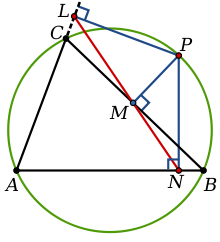
\includegraphics[width=10em]{res/Simson.png}
	\end{figure}

	以$ AB$中点为原点,$AB$方向为正方向,设$ A(-x_a,0),$ $B(x_a,0),$ $C(x_c,y_c),$ $P(x_p,y_p),$ $N(x_p,0),$ $M(x_m,y_m),$ $L(x_l,y_l)$.
	其条件可以化为如下代数方程组:
	\[  \begin{cases}
		PABC\texttt{共圆} &\Leftrightarrow y_cy_p^2-(y_c^2+x_c^2-x_a^2)y_p+y_c(x_p^2-x_a^2) =0\\
		PM\perp BC &\Leftrightarrow (x_c+x_a)(x_m-x_p)+y_c(y_m-y_p) =0\\
		M \in BC &\Leftrightarrow (x_c + x_a)y_n - y_c(x_n+x_a) =0\\
		PL \perp AC &\Leftrightarrow (x_c-x_a)(x_l-x_p) + y_c(y_l-y_p) = 0\\
		L \in AC &\Leftrightarrow (x_c-x_a)y_l - y_c(x_l-x_a)  = 0
	\end{cases}\]

	结论可写为: 
	$ (x_n-x_p)y_l - y_c(x_l-x_p) = 0$

	要证明原题结论,即证明上式在原方程组的生成理想中.
	吴文俊院士提出的机器证明方法,就是针对平面几何问题的特殊性提出的判断一多项式是否属于一个理想的快速方法.

\subsection{计算机图形学中的曲面拼接}
	在本学期选修的计算机系"计算机图形学基础"课程中,作者了解到多项式方程组求解在计算机几何造型的曲面拼接中的重要作用.

	对于一个参数曲面,传统的分析学中对连续性的定义不适用于图形学中
	,考虑参数方程表示的以下曲线\footnote{此例改编自胡事民老师"计算机图形学基础"课件}:
	\[  f(t) = \begin{cases} \dfrac{\overrightarrow X - \overrightarrow Y}{3}t,0\le t \le 1 \\
		\dfrac{\overrightarrow X - \overrightarrow Y}{3} + (t-1)\dfrac{2(\overrightarrow X - \overrightarrow Y)}{3},1 \le t \le 2
	\end{cases}\]

	参数连续性(Parametric Continuity)$ C^n $ 要求在各点的$ \dfrac{d^n f}{dt^n}$连续
	\footnote{详见\url{http://en.wikipedia.org/wiki/Smooth_function\#Parametric_continuity}}.
	在此例中,$ f'(1^-) \ne f'(1^+)$,因此在1处不满足$ C^1$连续,但事实上此函数图像为一直线.

	几何连续性(Geometric Continuity)$ G^n$忽略了参数在曲线上变化的速率,更适合描述图形学中的连续性.
	设$ P$点是曲面$ F_1 = 0, F_2 = 0$的一个公共点,
	若存在$ P$处非零的多项式$ A,B$使得$ AF_1-BF_2$的前$ k$阶导数均为0,则称两曲面在$ P$处$ G^k$连续.

	曲面拼接问题,就是对曲面$ F_1$与一辅助平面$ H=0$的交线$ C$,求曲面$ F_2$,使得$ F_2$与$ F_1$在$ C$上$ G^k$连续.
	其等价条件为, $ \exists \texttt{多项式}A,B,F_2 = AF + BH^{k+1}$,即$ F_2$在$ F_1$与$ H^{k+1}$的生成理想中\cite{warren}.
	因此这仍然是一个多项式代数的问题.

% $File: summary.tex
% $Date: Sat Jun 02 17:47:54 2012 +0800
% Author: Yuxin Wu <ppwwyyxxc@gmail.com>
\section{总结与感悟}
	本篇报告介绍了多项式方程组求解的结式方法,
	利用线性代数中的一些简单手段,就可以通过构造矩阵实现两个方程间的联合消元,
	进一步可以实现方程组的消元.
	随后,我们简要提及了更高效的抽象代数方法中的几个有价值的概念,
	将其与线性代数中的一些基本概念进行类比,加深了我们对这些代数概念的理解.

	20世纪以来现代科学技术突飞猛进,尤其是计算机科学的兴起为数学插上了腾飞的翅膀,
	数学理论同时也为计算机科学技术提供了广阔的舞台.
	现代的计算机技术为大型的符号计算提供了可能性,
	关键的问题就在于如何把抽象的代数理论算法化, 
	使计算机高效地处理形形色色的代数问题. 
	如今强大的计算机代数系统不仅是各类工程技术的助手,
	对纯粹科学研究也起着不可忽略的推动作用.
	在多项式代数理论上发展的计算机图形学,机器人运动学,密码学
	等一系列计算机专业相关领域和理论应运而生,
	也大规模的应用在我们的日常生活中.
	数学的规模之大,影响之深远,已经超越了所有的时代.
	虚拟现实,三维真实感动画,智能机械手臂等华丽实用的科技让人们切实感受到了数学博大精深,
	以及那种浑然天成的和谐美与对称美.
	
	这次接触计算机与数学领域重叠部分的前沿应用,
	既为未来的我们在计算机系的符号计算领域的学习打下基础,
	也有益于我们对已有的线性代数知识的理解和巩固.
	同时,在尝试用宏观和类比的眼光透视数学问题的过程中,我们也更加体会到了数学的美感,
	以及从变化中抓住不变,从紊乱中归纳条理,在偶然中发现必然,从混沌中整理秩序的科研精神.
	在完成这篇作品的过程中,
	从确定方向,查阅文献,类比研讨,抽象方法,再到研究实践应用的一系列过程里,我们感受到:
	在处理数学问题时要善于类比联想;由想激疑,在释疑中启悟;由疑反思,在思辨中省悟;由思导验,在体验中领悟;由验致用,在应用中彻悟。

\printbibliography
%\input{appendix.tex}

\end{document}

